\documentclass[a4paper, 12pt]{article}
\usepackage[T2A]{fontenc}
\usepackage[utf8]{inputenc}
\usepackage[english,russian]{babel}
\usepackage{amsmath, amsfonts, amssymb, amsthm, mathtools, misccorr, indentfirst, multirow}
\usepackage{wrapfig}
\usepackage{graphicx}
\usepackage{subfig}
\usepackage{adjustbox}
\usepackage{pgfplots}
\usepackage{mathrsfs}

\usepackage{geometry}
\geometry{top=20mm}
\geometry{bottom=20mm}
\geometry{left=20mm}
\geometry{right=20mm}
\newcommand{\angstrom}{\textup{\AA}}
\begin{document}
	\title{Лабораторная работа №11.1\\Определение ширины запрещенной зоны полупроводников.}
	\author{Нехаев Александр 654гр.}
	\maketitle
	\tableofcontents
	\section{Введение}
	\paragraph{Цель работы}
	Исследовать температурную зависимость проводимости типичного полупроводника (германия или кремния). Определить ширину запрещенной зоны с помощью универсального вольтметра.
	\subsection{Теоретические основы}
	Величина электропроводности в полупроводниках определяется числом электронов в зоне проводимости и дырок в валентной зоне (эти числа в чистыъ полупроводниках, конечно, равны друг другу).

	Число электронов, находящихся в зоне проводимости, равно произведению числа имеющихся уровней на вероятность их заполнения. Вероятность заполнения уровней определяется функцией Ферми, которая в нашем случае мало отличается от простого экспоненциального больцмановского распределения:
	\begin{equation}
		f(E) = \frac{1}{\exp\left(\frac{E-\mu}{k_{\text{Б}}T}\right)+1}\simeq\exp{\left(-\frac{E-\mu}{k_{\text{Б}}T}\right)},
		\label{FermiFunc}
	\end{equation}
	так как $(E-\mu)\gg k_{\text{Б}}T$.

	В формулу (\ref{FermiFunc}) $E$ -- энергия уровня в зоне проводимости, $\mu$ -- некоторая константа, которая, вообще говоря, зависит от температуры и называется энергией или уровнем Ферми. В собственных полупроводниках энергия Ферми лежит вблизи середины запрещенной зоны.

	При не очент высоких температурах заняты главным образом уровни, находящиеся у дна зоны проводимости, так что в качестве энергии $E$ можно подставить энергию $E_c$, соотвествующую дну зоны проводимости. При этом вместо полного числа уровней в зоне нужно подставлять некоторое эффективное число уровней $Q_n$, находящихся вблизи дна зоны, тогда число электронов в зоне проводимости будет равно\footnote{Строго говоря, число $Q_n$ выбирается так, чтобы равенство (\ref{electronsAmount}) давало правильное число электронов при подстановке энергии дна зоны $E_c$ вместо энергии $E$.}:
	\begin{equation}
		n_n=Q_n\exp{\left(-\frac{E_c-\mu}{k_{\text{Б}}T}\right)}.
		\label{electronsAmount}
	\end{equation}

	Вероятность появления дырки в валентной зоне определяется разностью $1-f(E)$. Поэтому число дырок равно
	\begin{equation}
		n_p=Q_p\left[1-\frac{1}{\exp{\left(\frac{E_v-\mu}{k_{\text{Б}}T}\right)+1}}\right]\simeq Q_p\exp{\left(-\frac{E_v-\mu}{k_{\text{Б}}T}\right)}.
		\label{holesAmount}
	\end{equation}

	При преобразованиях формулы (\ref{holesAmount}) было принято во внимание, что энергия верхнего края валентной зоны $E_v$ меньше $\mu$ и дробь $(E_v-\mu)/(k_{\text{Б}}T)$ является большим отрицательным числом.

	Перемножим формулы (\ref{electronsAmount}) и (\ref{holesAmount}) и примем во внимание, что число электронов равно числу дырок:
	\begin{equation}
		n_nn_p=n^2=Q_nQ_p\exp{\left(-\frac{E_c-E_v}{k_{\text{Б}}T}\right)}.
		\label{n^2:eq}
	\end{equation}

	Разность $E_c-E_v$ равна ширине запрещенной зоны $\Delta$. Обозначая для краткости произведение
	\begin{equation}
		Q_nQ_p=C^2
	\end{equation}
	и извлекая квадратный корень из (\ref{n^2:eq}), получим
	\begin{equation}
		n=C\exp{\left(-\frac{\Delta}{2k_{\text{Б}}T}\right)}.
		\label{eq:n}
	\end{equation}

	Найдем теперь электропроводность полупроводника. В присутствии поля, большая часть электронов в зоне проводимости начинает двигаться в сторону, противоположную полю. Средняя величина скорости электронов перестает быть равной нулю и направлена вдоль поля. При этом вплоть до самых сильных полей (практически до пробоя) справедлива формула
	\begin{equation}
		v_{\text{ср}}=\mu_n\mathscr{E},
		\label{avgSpeed}
	\end{equation}
	где $v_{\text{ср}}$ -- среднее значение дрейфовой скорости электронов, $\mathscr{E}$ -- напряженность электрического поля, $\mu_n$ -- коэффициент пропорциональности, носящий название подвижности электронов; он определяет, какую среднюю скорость приобретает электрон в поле единичной напряженности (обычно численное значение подвижности приводят для поля 1 В/см).

	Применяя формулу (\ref{avgSpeed}) к электронам в зоне проводимости и к дыркам в валентной зоне, найдем, обозначая через $j=nev_{\text{ср}}$ плотность электрического тока, что
	\begin{equation}
		\sigma=j/\mathscr{E}=|e|(n_n\mu_n+n_p\mu_p).
		\label{sigmaDefenition}
	\end{equation}
	
	Подставляя в (\ref{sigmaDefenition}) значение $n_n=n_p$ из (\ref{eq:n}), получим
	\begin{equation}
		\sigma=|e|C\left(\mu_n+\mu_p\right)\exp{\left(-\frac{\Delta}{2k_{\text{Б}}T}\right)}=A\exp{\left(-\frac{\Delta}{2k_{\text{Б}}T}\right)},
		\label{mainEq}
	\end{equation}
	где предэкспоненциальный множитель заменен константой\footnote{Более точные расчеты показывают, что величина $A$ зависит от температуры. Этой зависимостью, однако, можно пренебречь по сравнению с быстро изменяющейся экспонентой.}.

	Измерим электропроводность $\sigma$ как функцию температуры и изобразим результаты на графике в полулогарифмическом масштабе:
	\begin{equation}
		\ln\sigma=f(1/T).
		\label{graphEq}
	\end{equation}

	Формула (\ref{mainEq}) показывает, что график должен иметь вид прямой линии с наклоном $\Delta/(2k_{\text{Б}})$. Наклон прямой (\ref{graphEq}) позволяет, таким образом, определить ширину запрещенной зоны.
	\subsection{Схема установки}
	\begin{figure}[!htb]
		\centering
		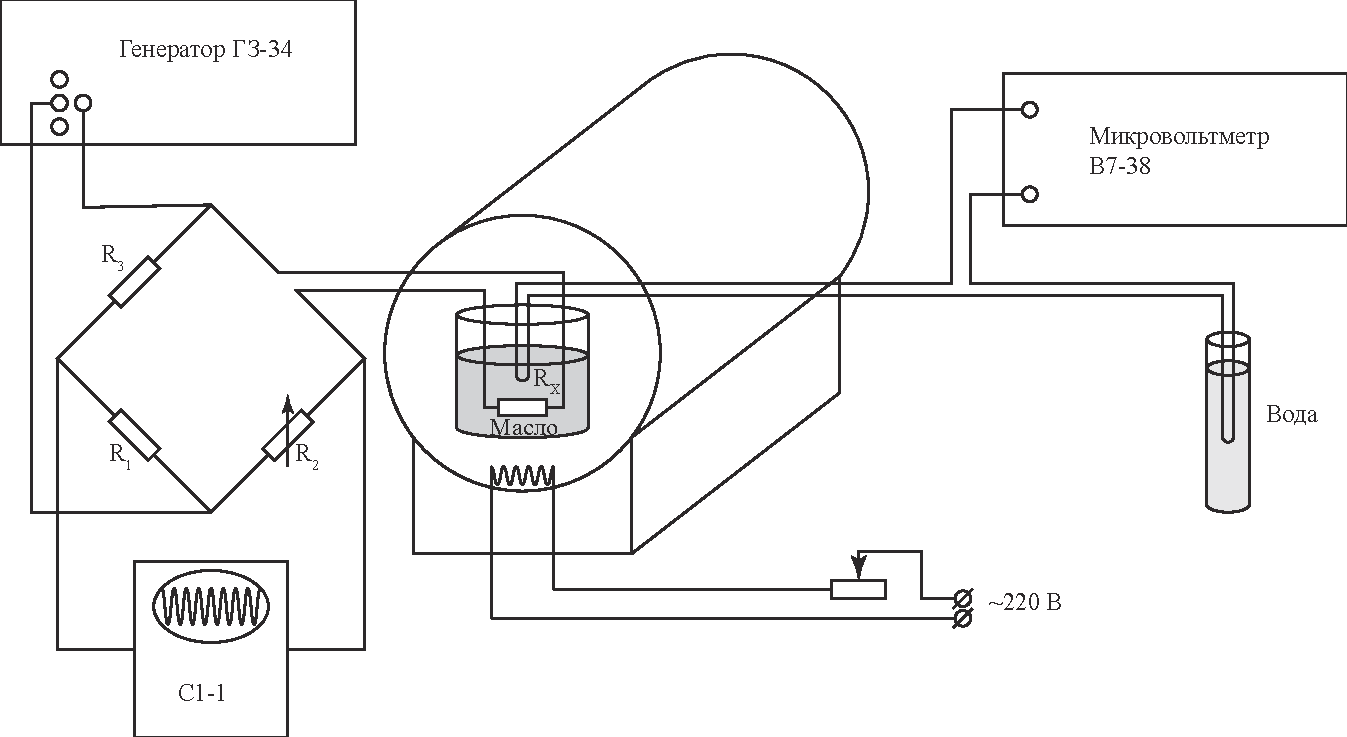
\includegraphics[scale=0.6]{scheme.pdf}
		\caption{Схема установки}
	\end{figure}
	Температура второго спая термопары измеряется спиртовым термометром, помещенным в сосуд дьюара. Рекомендуемый режим работы: частота -- 500-700 Гц, усиление -- $\frac{1}{2}$ шкалы, затухание -- 10 дБ, $R_1=220$ Ом, $R_3=560$ Ом. Чувствительность термопары: $41\cdot10^{-6}$ В/град.
	\begin{figure}[!htb]
		\centering
		\includegraphics[scale=0.2]{box.png}
		\caption{Геометрические размеры образца}
	\end{figure}
	\section{Ход работы}
	Проводим измерение сопротивления образцов в зависимости от температуры, данные о которой берем из значения напряжения на термопаре. Начальное значение термопары 100 мкВ при температуре 300.6 К. Используя формулу $\sigma=\frac{l}{RS}$, строим график $\sigma(T)$.
	\begin{figure}[!htb]
		\centering
		\includegraphics[scale=1]{graph1.pdf}
		\caption{График зависимости $\sigma(T)$.}
	\end{figure}

	Подобный вид зависимости объясняется природой материала, определяющение эти законы.
	\begin{equation}
		\sigma=|e|C(\mu_n+\mu_p)\exp{\left(-\frac{\Delta}{2kT}\right)}
	\end{equation}

	Строим график $\ln(\sigma)=f(1/T)$. Зная, как представляется эта зависимость по наклону прямой получаем, что ширина запрещенной зоны $\Delta=0,69$ эВ. 
	\begin{figure}[!htb]
		\centering
		\includegraphics[scale=1]{graph2.pdf}
		\caption{График зависимости $\ln(\sigma)=f(1/T)$}
	\end{figure}

	\section{Вывод}
	В ходе лабораторной работы удалось предложенным методом измерить ширину запрещенной зоны полупроводника -- $\Delta=0.69$ эВ, что позволяет сделать вывод о природе исследумого материала. Полученное значение соотвествует ширине запрещенной зоны германия (0.67 эВ).
\end{document}